\documentclass[12pt]{article}
\setlength{\parskip}{0.2cm}
\setlength{\parindent}{0.5cm}
 
\usepackage[margin=1in]{geometry} 
\usepackage{amsmath,amsthm,amssymb}
\usepackage{graphicx}
\usepackage[english]{babel}
\usepackage{hyperref}
\usepackage{subcaption}

\begin{document}


\title{Homework 3 - Report}
\author{Álvaro Martínez Alfaro\\
    Autonomous Robotics}

\maketitle

\section{Introduction}

The objective of this assignment is to develop and integrate a trajectory-tracking control system for
an autonomous agent operating within the \textit{ROS2} \texttt{turtlesim} environment. The primary
task requires the robot to continuously navigate a predefined closed-loop track, composed of two
straightaways and two semi-circular curves with a radius of $r = 2$, at a constant linear velocity
of $v_x=0.2$ units per second. The controller governs the agent's heading by calculating the
appropriate angular velocity to minimize the \textbf{cross-track error} (CTE) relative to the
guidance path.

To achieve this, a \textbf{Proportional-Derivative} (PD) controller was implemented. The PD
controller is a continuous feedback mechanism that computes an error value as the difference between
the track center and the robot's current position, applying a restorative correction.

Formally, let $cte_t$ denote the CTE at time $t$, defined as the orthogonal distance from the robot's
origin to the target trajectory. The control law is defined as:
\begin{equation}
    \delta_t = -\tau_p \cdot cte_t - \tau_d \cdot \frac{cte_t-cte_{t-1}}{\Delta t}
\end{equation}
where $\tau_p$ generates a restorative force directly proportional to the current error magnitude
and $\tau_d$ generates a control signal proportional to the instantaneous rate of change of the
error.

This report details the implementation of this control architecture, focusing on the advanced
development requirement: the dynamic optimization of the hyperparameters $\tau_p$ and $\tau_d$ by
exploring the parameter space over consecutive laps to minimize the aggregate error.

%------------------------------------------------

\section{Advanced development}

The advanced implementation of this assignment focuses on two main improvements over the base
controller: increasing the control loop frequency for greater stability and implementing a coordinate
descent algorithm (\textbf{Twiddle}) to optimize the hyperparameters $\tau_p$ and $\tau_d$.

One implementation detail is that the base implementation forces the \texttt{listener\_callback} to
execute only once per second. This limitation was reduced to $0.1$ seconds, allowing the robot to
correct its orientation more frequently.

\subsection{Cross-Track Error (CTE) computation}

To provide accurate feedback to the controller, the track is partitioned into four regions. The CTE
is calculated differently depending on the robot's spatial coordinates $(x,y)$:

\begin{enumerate}
    \item \textbf{Top straightaway}: for $x \in [3.5, 7.5]$ and $y > 5.5$, the reference trajectory
          is the horizontal line $y_{ref} = 7.5$. The error is calculated as $CTE = y - y_{ref}$.
    \item \textbf{Bottom straightaway}: for $x \in [3.5, 7.5]$ and $y \leq 5.5$, the reference is
          $y_{ref} = 3.5$, and the error is $CTE = y_{ref} - y$.
    \item \textbf{Left curve}: for $x < 3.5$, the reference is a semicircle centered at $(3.5, 5.5)$
          with $r = 2.0$. Using the \textit{Euclidean} distance metric, $CTE = \sqrt{(x-3.5)^2 + (y-5.5)^2} - r$.
    \item \textbf{Right curve}: for $x > 7.5$, the reference is a semicircle centered at $(7.5, 5.5)$
          with $r = 2.0$, and the error is $CTE = \sqrt{(x-7.5)^2 + (y-5.5)^2} - r$.
\end{enumerate}

These calculations ensure that a positive CTE indicates the robot is outside the track, while a
negative CTE indicates it has drifted inside the track.

\subsection{Hyperparameter optimization}

Instead of relying on static values for $\tau_p$ and $\tau_d$, the system utilizes the \textbf{Twiddle}
algorithm to search the parameter space for an optimal configuration. Twiddle is a local search
optimization algorithm that iteratively adjusts one parameter at a time and evaluates the resulting
system performance.

The cost function to be minimized is the Average Absolute CTE per lap, defined as:
\begin{equation}
    J(\tau_p, \tau_d) = \frac{1}{N} \sum_{i=1}^{N} |cte_i|
\end{equation}
where $N$ is the number of callbacks processed during a lap. A lap is considered complete when the
robot crosses the vertical midline at $x = 5.5$ in the positive direction within the top straightaway,
guarded by a 2-second cooldown to prevent possible redundant triggers.

Furthermore, the Twiddle algorithm maintains a tuning vector $p = [\tau_p, \tau_d]$ and a step
vector $\Delta p$. After evaluating the baseline error on the first lap, the algorithm enters a
continuous state machine at the end of every lap, adjusting the parameters as follows:
\begin{enumerate}
    \item \textbf{Exploration} (state 0): The algorithm increases the parameter space by adding
          $\Delta p_i$ to the current parameter $p_i$. If $J(p)$ improves, the modification is kept,
          the step size is increased ($\Delta p_i \leftarrow 1.1 \cdot \Delta p_i$) to accelerate
          convergence, and the algorithm moves to the next parameter. Otherwise, if the error
          increases, the algorithm subtracts $2 \cdot \Delta p_i$ to probe the opposite direction
          and shifts to state 1.
    \item \textbf{Reversion} (state 1): if the opposite direction yields a lower error, the change
          is kept, and the step size is increased. If both directions result in a higher error than
          the historical best, the parameter is reverted to its original state, and the step size is
          reduced ($\Delta p_i \leftarrow 0.9 \cdot \Delta p_i$) to refine the search resolution.
\end{enumerate}

To visualize the optimization process, the system leverages an aynchronous ROS service call
(\texttt{/turtle/set\_pen}) to change the robot's trajectory color at the start of a new lap. It
is asynchronous to avoid blocking the control loop.

%------------------------------------------------

\section{Results}

To evaluate the efficacy of the dynamic parameter optimization, the simulation was executed for 15
consequtive laps. The robot's initial spatial configuration was set to
$(x_0, y_0, \theta_0) = (3.5, 7.5 \pm 0.5, r)$, where $r$ is a random angle in the range $[-0.2, 0.2]$.

The controller was initialized with the baseline parameters $\tau_p = 0.4$ and $\tau_d = 0.6$. To
initialize the local search, the Twiddle step sizes were set to $\Delta p_p = 0.05$ and $\Delta p_d = 0.05$.
During the first lap, the system operated strictly with these parameters to establish a performance
baseline, yielding an average absolute CTE of $J_{baseline} = 0.1716$.

\subsection{Analysis of convergence}

Following the initial lap, the descent algorithm activated. The Figure \ref{fig:convergence} illustrates
the parameter space exploration and the corresponding reduction in the objective function $J$ over time.

% \begin{table}
%     \centering
%     \caption{Evolution of PD parameters and average error per lap via Twiddle optimization.}
%     \label{tab:optimization}
%     \begin{tabular}{lccc}
%         \hline
%         \textbf{Lap} & \textbf{Average CTE ($J$)} & \textbf{Proportional Gain ($\tau_p$)} & \textbf{Derivative Gain ($\tau_d$)} \\
%         \hline
%         1 (Base)     & 0.1716                     & 0.4000                                & 0.6000                              \\
%         2            & 0.1560                     & 0.4500                                & 0.6500                              \\
%         3            & 0.1537                     & 0.5050                                & 0.6500                              \\
%         4            & 0.1378                     & 0.5050                                & 0.7050                              \\
%         5            & 0.1358                     & 0.5655                                & 0.7050                              \\
%         6            & 0.1219                     & 0.5655                                & 0.7655                              \\
%         7            & 0.1202                     & 0.6321                                & 0.7655                              \\
%         8            & 0.1081                     & 0.6321                                & 0.8321                              \\
%         9            & 0.1068                     & 0.7053                                & 0.8321                              \\
%         10           & 0.0961                     & 0.7053                                & 0.9053                              \\
%         11           & 0.0951                     & 0.7858                                & 0.9053                              \\
%         12           & 0.0860                     & 0.7858                                & 0.9858                              \\
%         13           & 0.0851                     & 0.8744                                & 0.9858                              \\
%         14           & 0.0770                     & 0.8744                                & 1.0744                              \\
%         Final        & 0.0763                     & 0.9718                                & 1.0744                              \\
%         \hline
%     \end{tabular}
% \end{table}

As observed, the Twiddle algorithm achieved a near-monotonic convergence, reducing the average CTE
from an initial baseline of approximately $0.17$ down to under $0.08$ by the final lap. Also,
modifications to $\tau_d$ caused more significant reductions in the error compared to adjustments in
$\tau_p$, indicating that the system's performance was more sensitive to the derivative term.

The parameter space search (Figure \ref{fig:convergence}, bottom) reveals a coupled dynamic between
the control gains. The algorithm consistently increased $\tau_p$ to minimize lateral drift along
the straightaways. Because unilaterally increasing $\tau_p$ typically induces oscillations, the
algorithm also increased $\tau_d$ to provide additional damping. This stair-step growth allowed the
controller to track the reference trajectory while mitigating overshoot in curved sections.
Furthermore, the lack of downward adjustments in the parameter values indicates a smooth descent
towards a local minimum without being destabilized.

\begin{figure}
    \centering
    \begin{subfigure}[b]{0.58\textwidth}
        \centering
        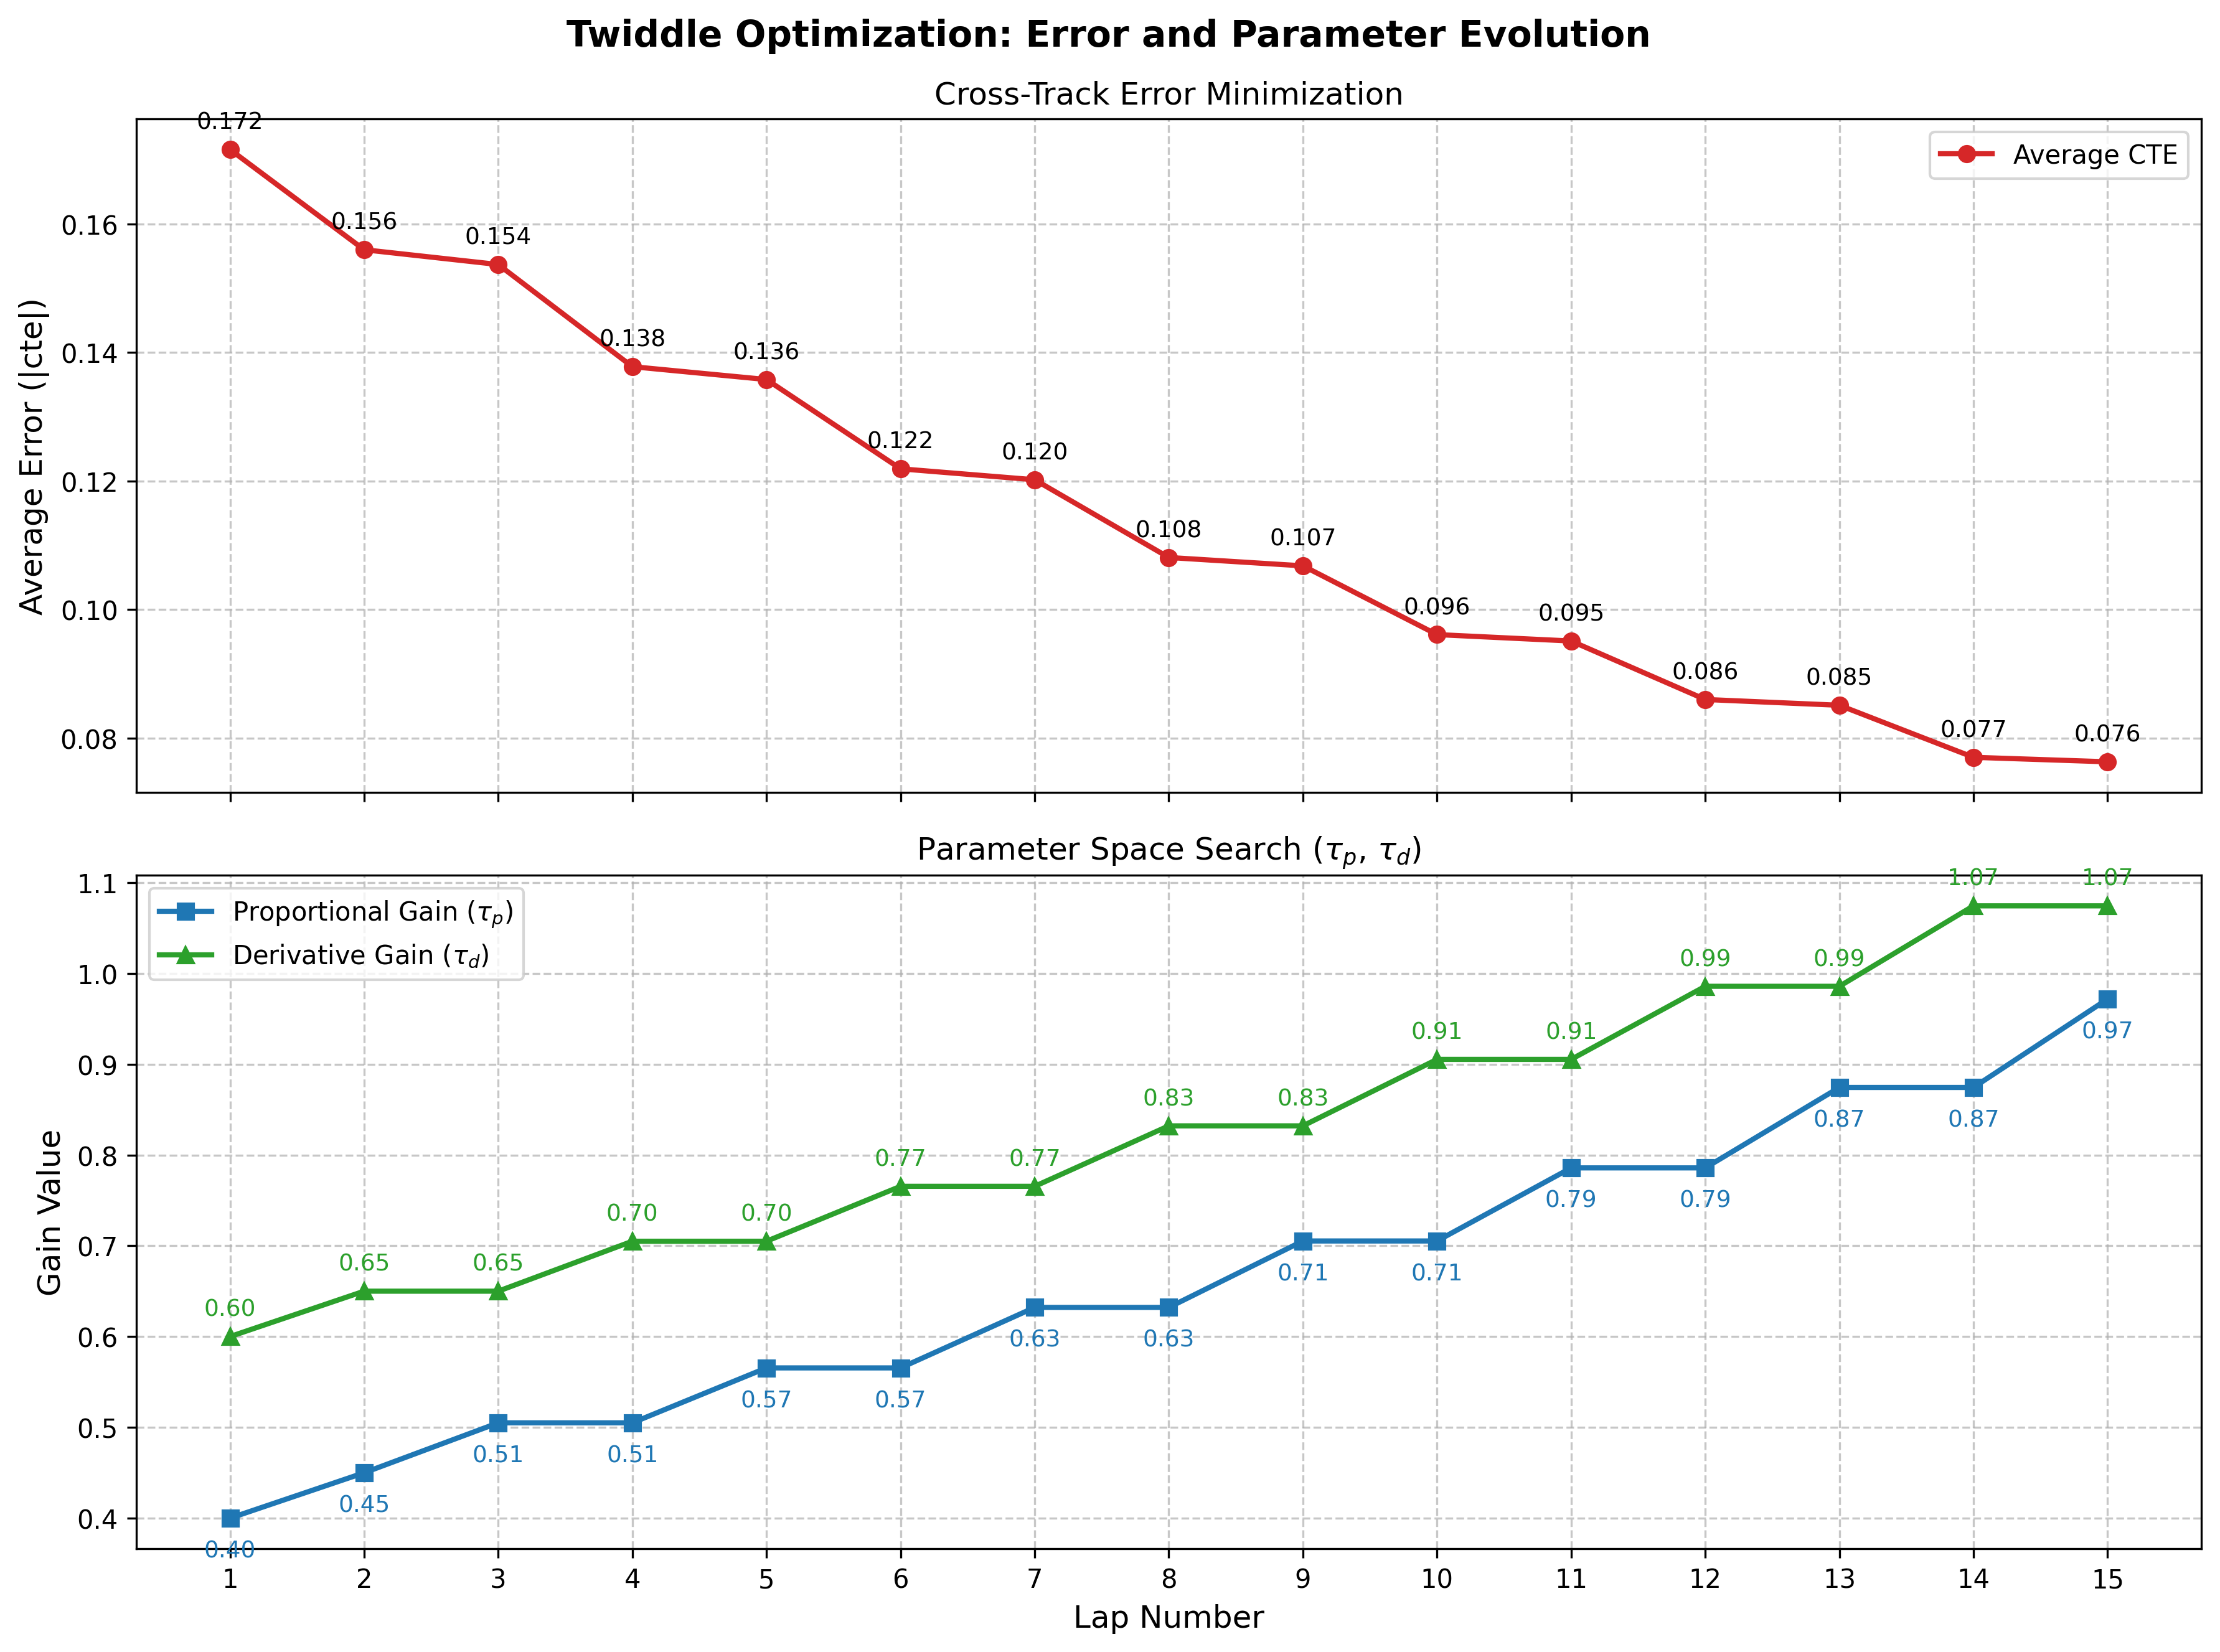
\includegraphics[width=\textwidth]{img/twiddle_results.png}
        \caption{Convergence of the average CTE over consecutive laps.}
        \label{fig:convergence}
    \end{subfigure}
    \hfill
    \begin{subfigure}[b]{0.3\textwidth}
        \centering
        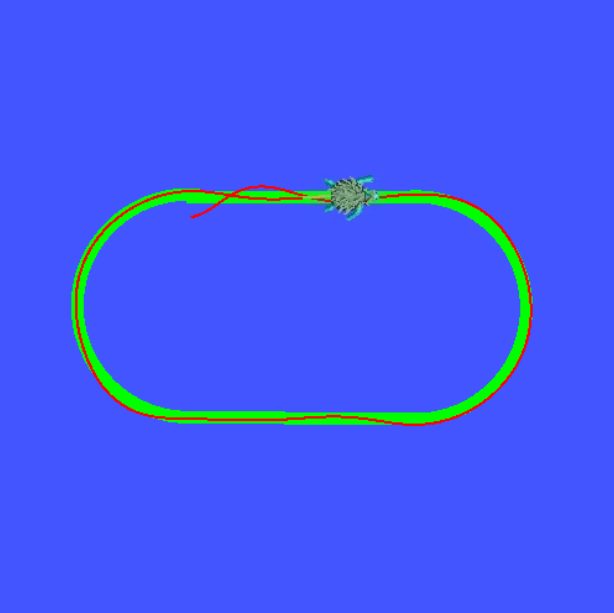
\includegraphics[width=\textwidth]{img/final_trajectory.png}
        \caption{Trajectory (optimized).}
        \label{fig:final_trajectory}
    \end{subfigure}

    \caption{Results of the dynamic parameter optimization.}
    \label{fig:combined_results}
\end{figure}

\subsection{Optimized trajectory validation}

To verify the effectiveness of the optimized parameters, the controller was initialized with the
final values $\tau_p = 0.9718$ and $\tau_d = 1.0744$ and executed for an additional lap.

Figure \ref{fig:final_trajectory} illustrates the spatial trajectory of the robot during the first
lap of this validation run. Unlike the baseline initialization which yielded an initial CTE of $0.17$,
the pre-optimized controller started with a significantly lower initial error of approximately $0.07$.

Visually, the trajectory closely adheres to the reference path. The elevated $\tau_d$ preempts the
transition points at ($7.5, 7.5$) and ($3.5, 3.5$), allowing the robot to enter the curves without
overshooting. This confirms that the hyperparameters represent a generalized optimal configuration
for this track geometry, rather than being overfitted.

%------------------------------------------------

\section{Conclusion}

This assignment has served as a good exercise to be introduced to the \textit{ROS 2} ecosystem and
to implement a basic PD controller for trajectory tracking. The advanced development requirement
pushed it further by integrating an optimization algorithm to tune the controller's hyperparameters
based on the robot's performance.

The system successfully reduced the average CTE from an initial $0.17$ to under $0.08$. Furthermore,
the final spatial validation confirmed that these optimized parameters yielded a more robust and
accurate trajectory tracking performance.

\end{document}
